\chapter{Effects of Image Generation Parameters}
\label{ch:appendix_image_generation}

This appendix contains additional figures demonstrating the effects of the sampler type, number of sampling steps, and CFG scale on the image generation process.
\\
\\
\\
\\
\\


\figure[!h]
    \centering
    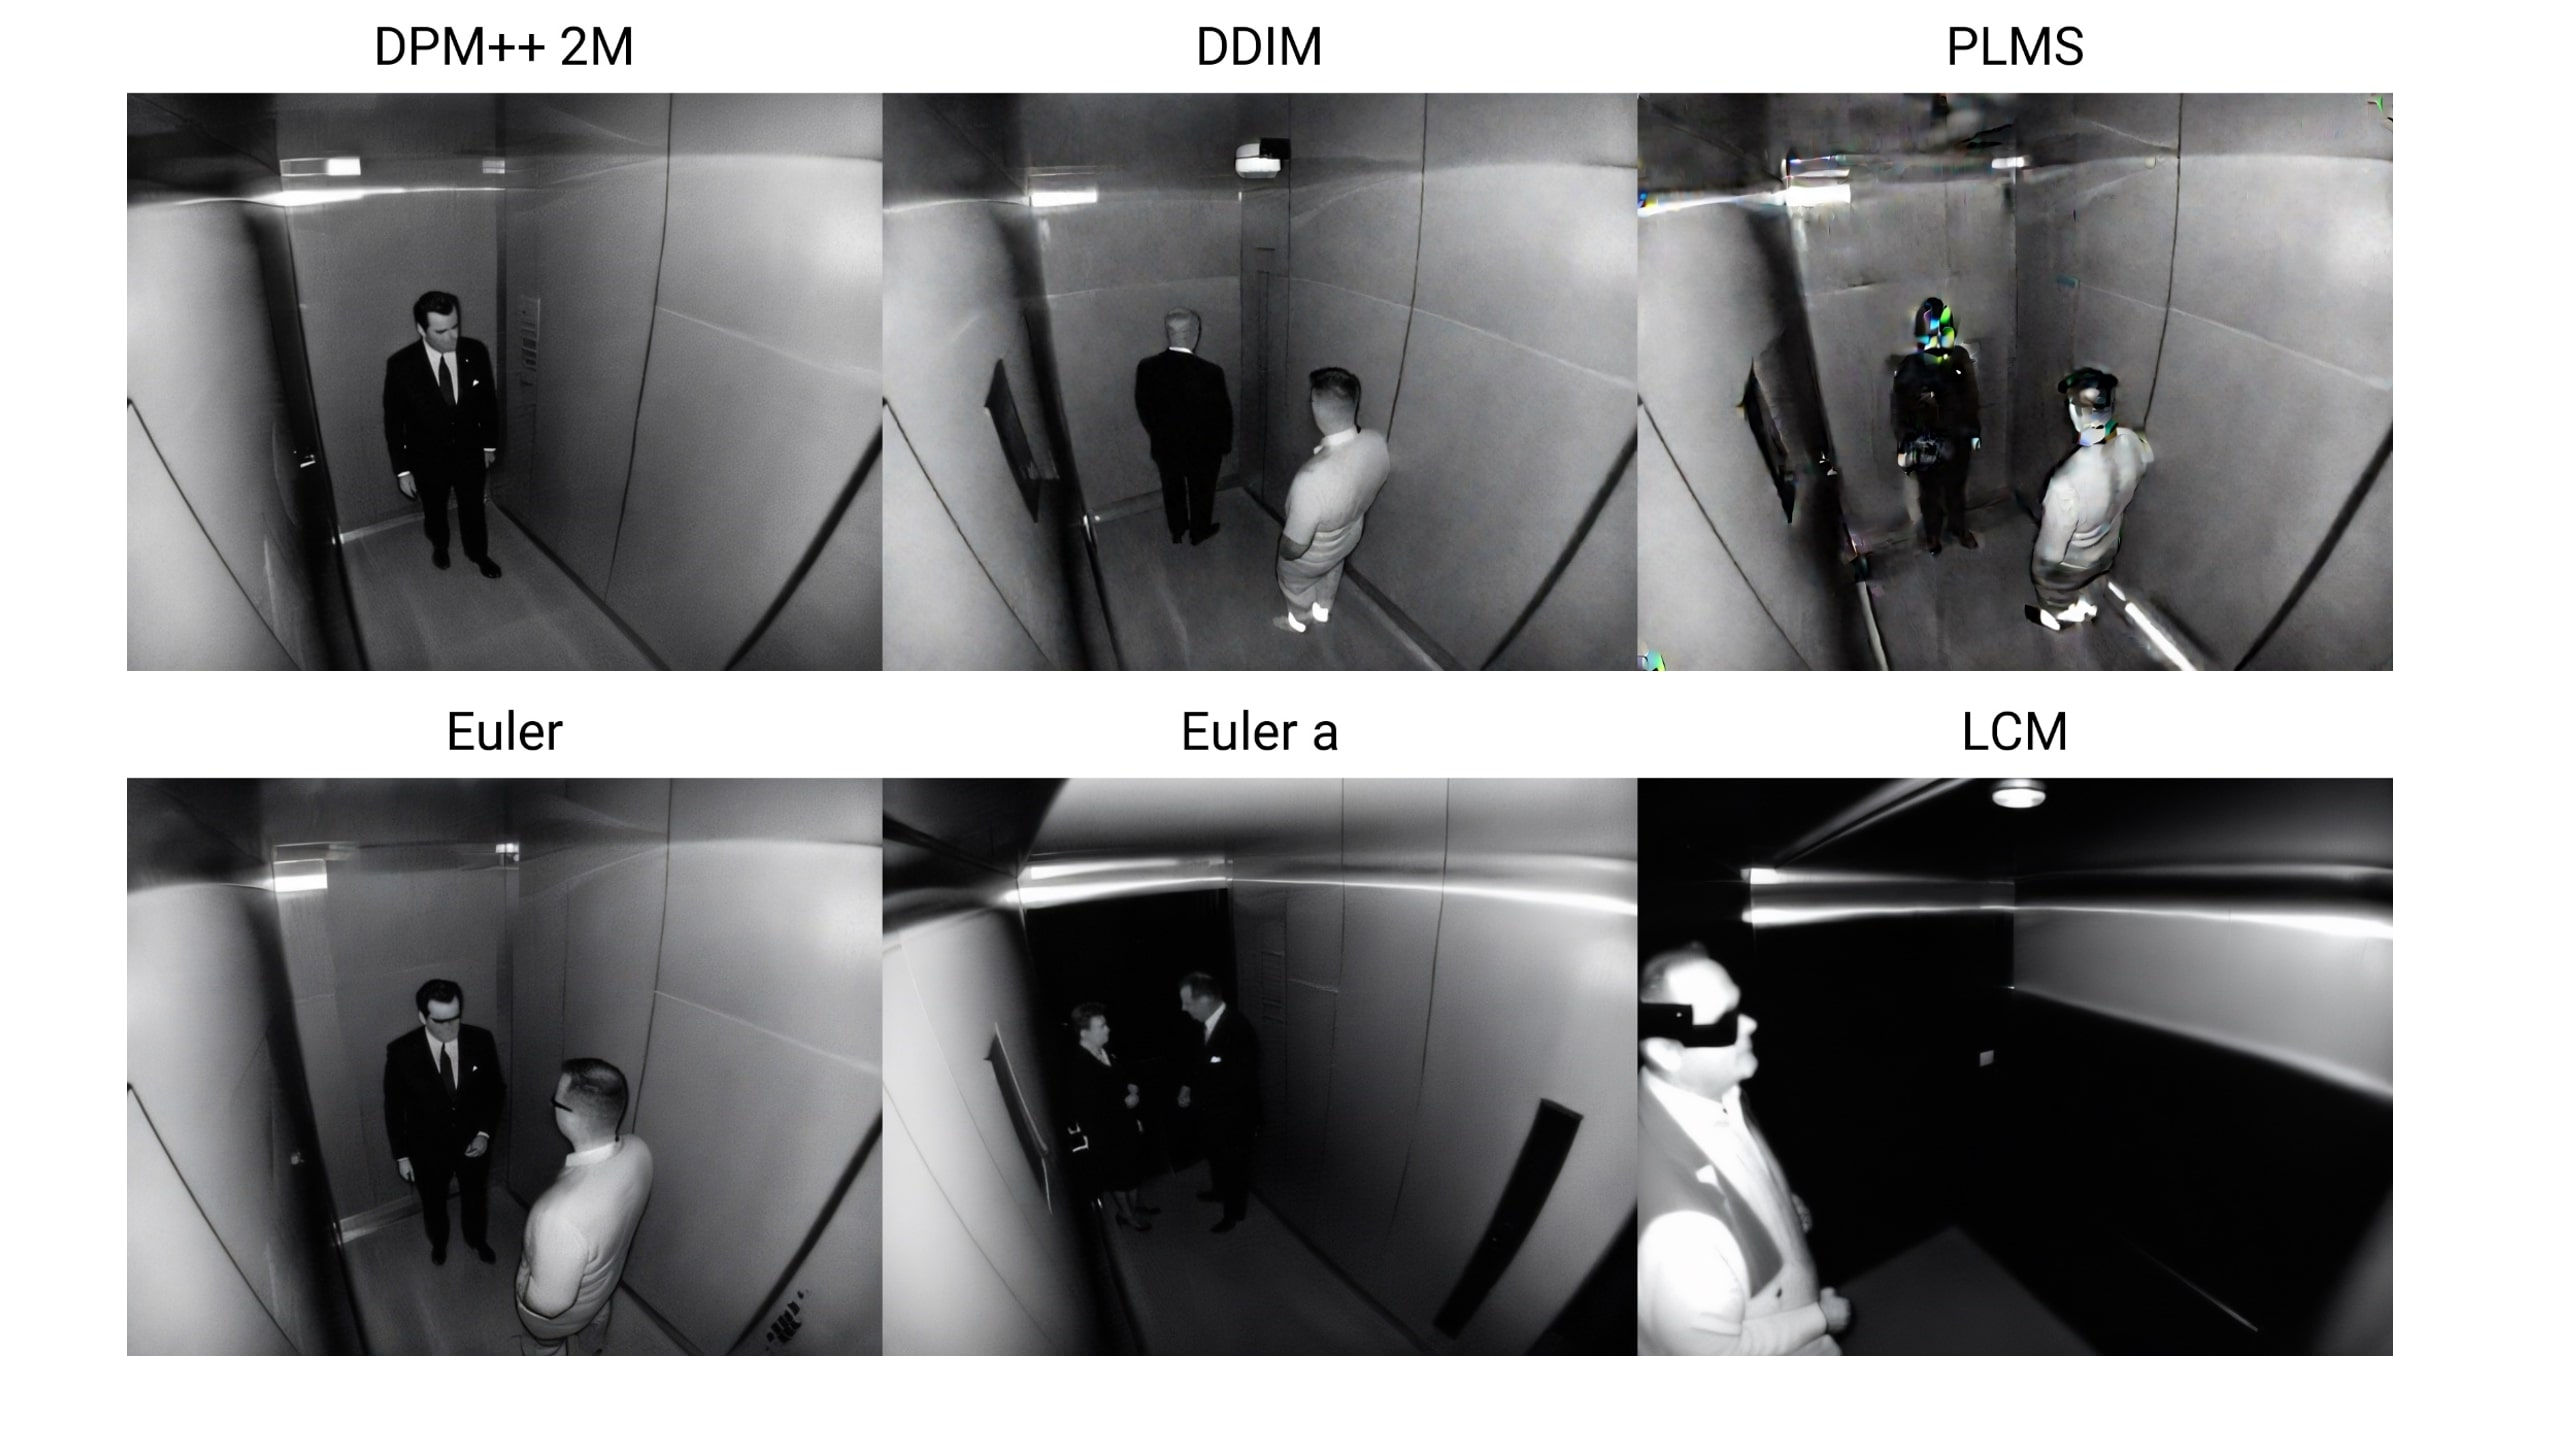
\includegraphics[width=1\textwidth]{images/methotologies/generation/sampler.jpg}
    \caption{Effect of changing the sampler while keeping the random seed and other parameters from Table~\ref{tab:imagegen_params} constant.}
    \label{fig:samplers}
\endfigure

\figure[!h]
    \centering
    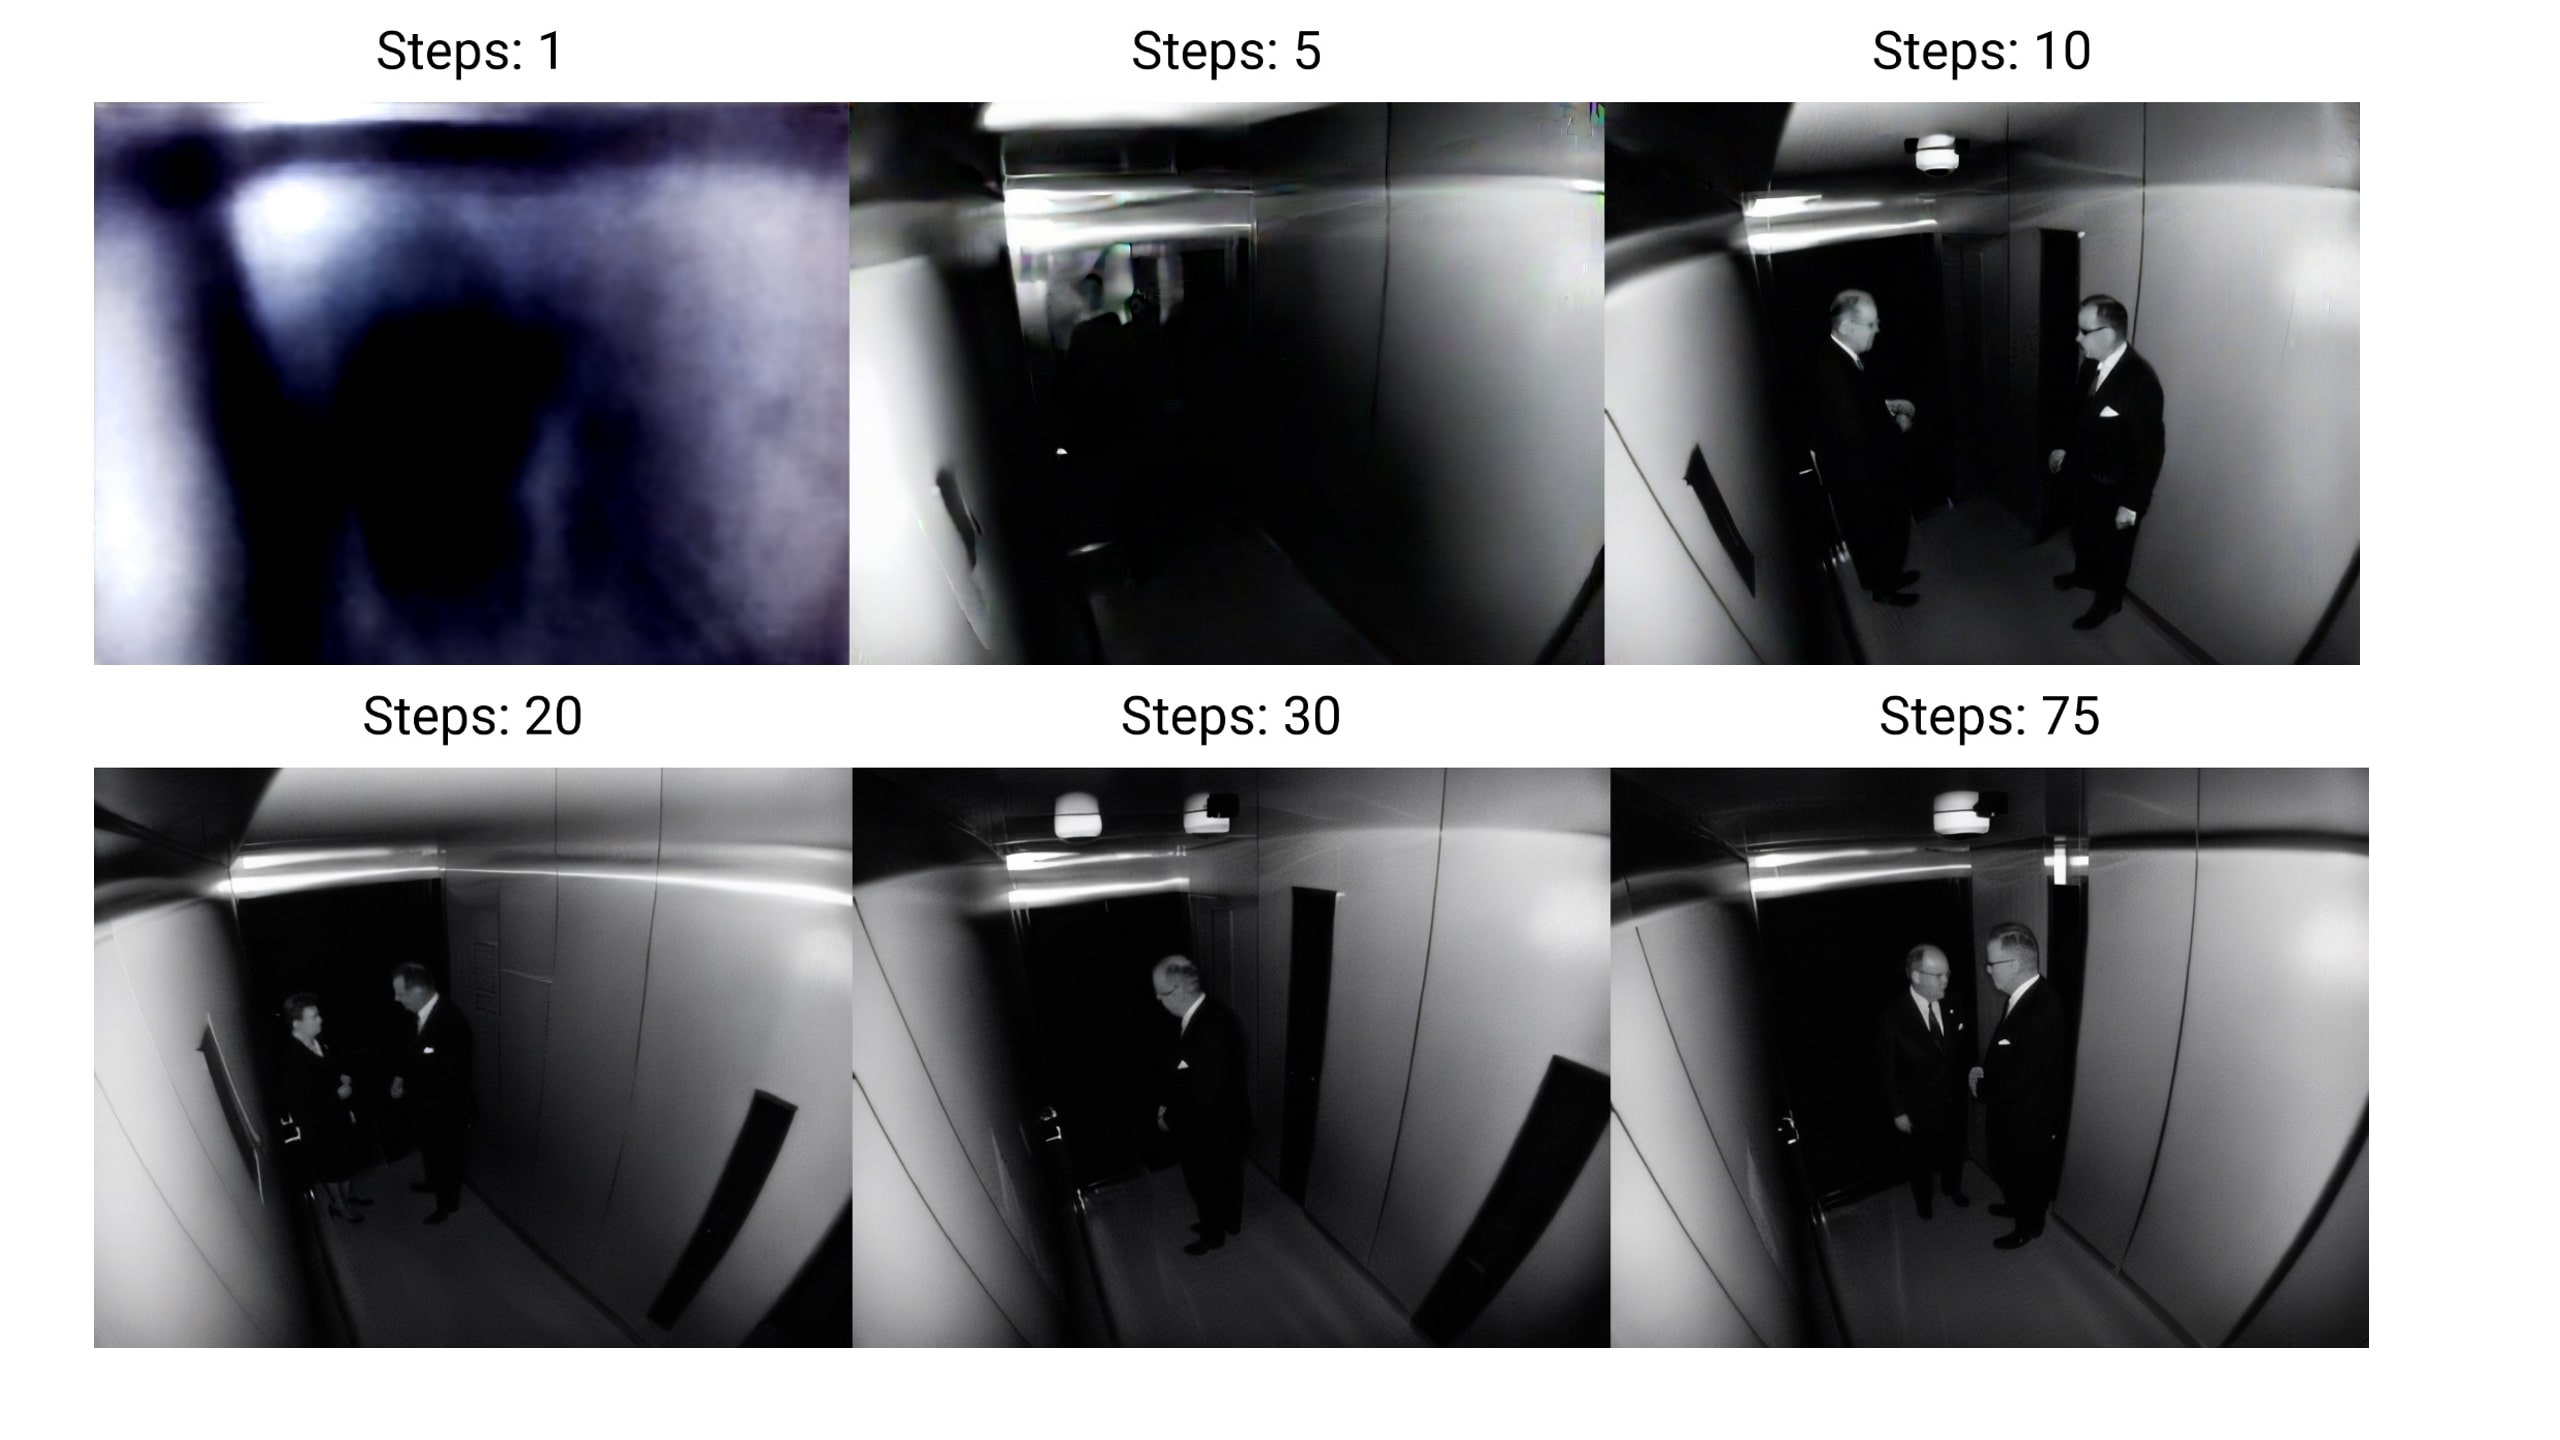
\includegraphics[width=1\textwidth]{images/methotologies/generation/steps.jpg}
    \caption{Effect of changing the sampling step while keeping the random seed and other parameters from Table~\ref{tab:imagegen_params} constant.}
    \label{fig:steps}
\endfigure

\figure[!h]
    \centering
    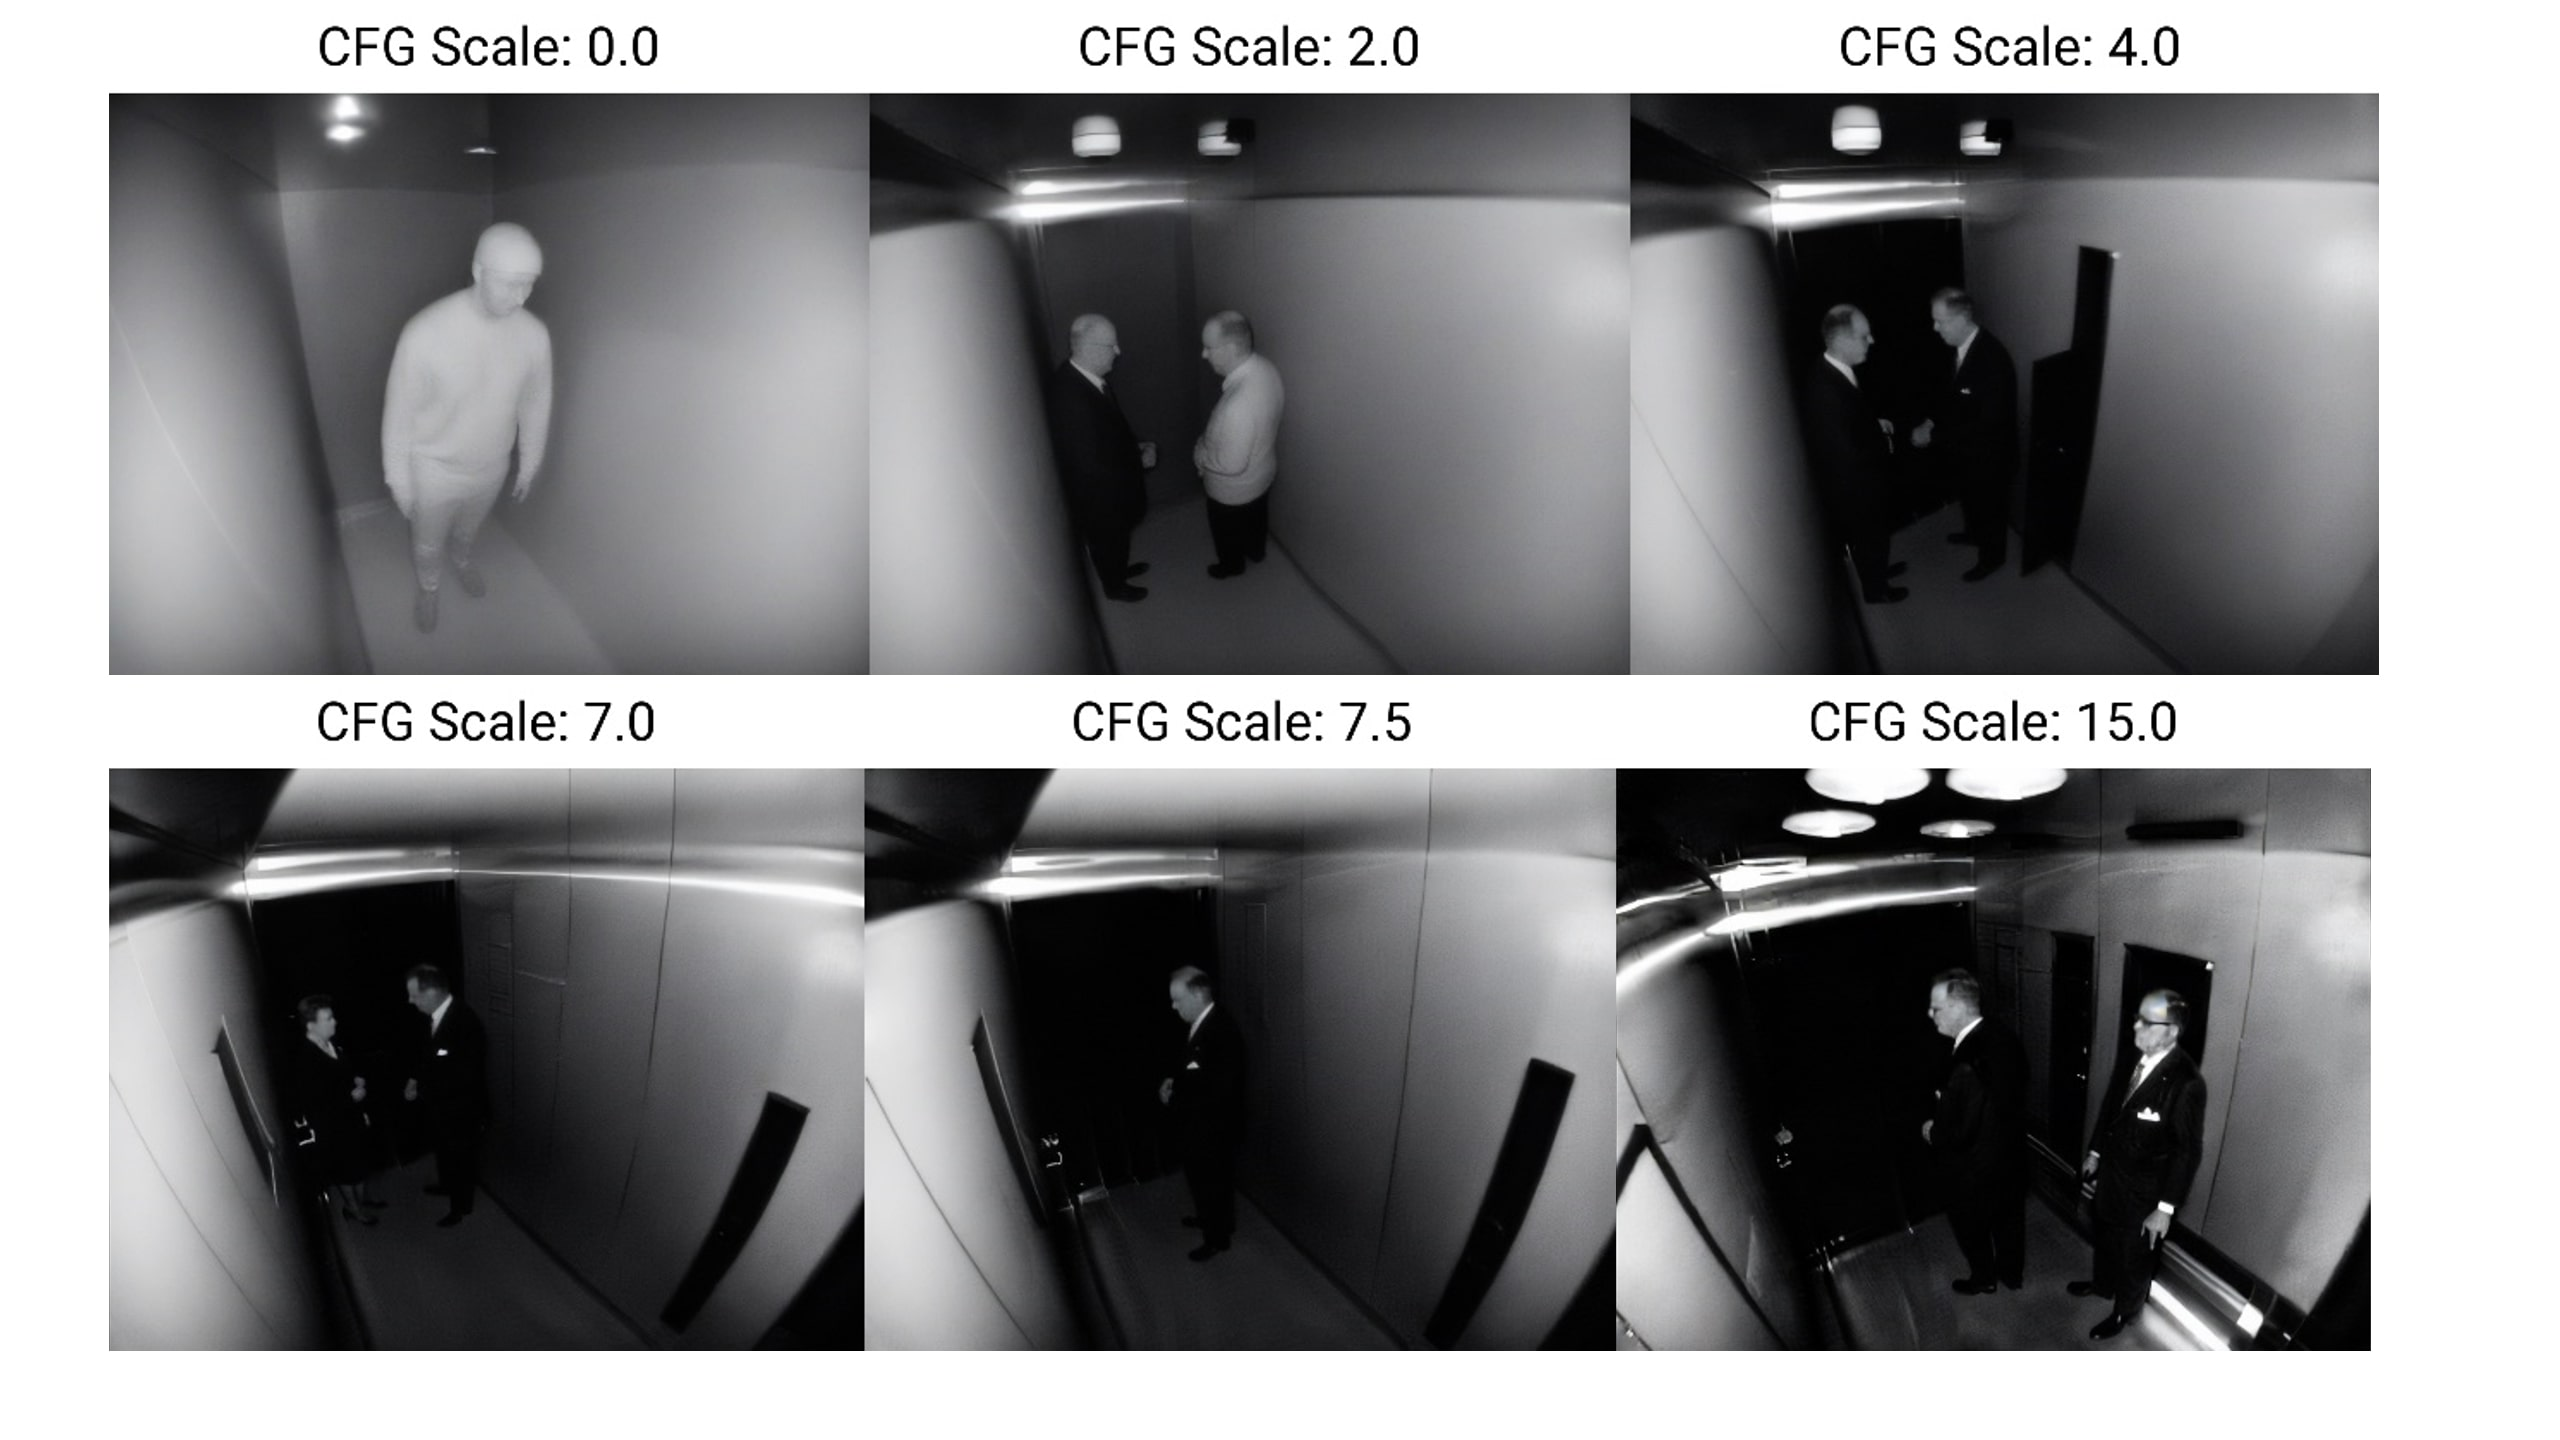
\includegraphics[width=1\textwidth]{images/methotologies/generation/CFG.jpg}
    \caption{Effect of changing the CFG while keeping the random seed and other parameters from Table~\ref{tab:imagegen_params} constant.}
    \label{fig:CFG}
\endfigure

    
\chapter{Additional Results}

This appendix contains additional results from the object detection model evaluation.

 \begin{figure}[ht]
    \centering
    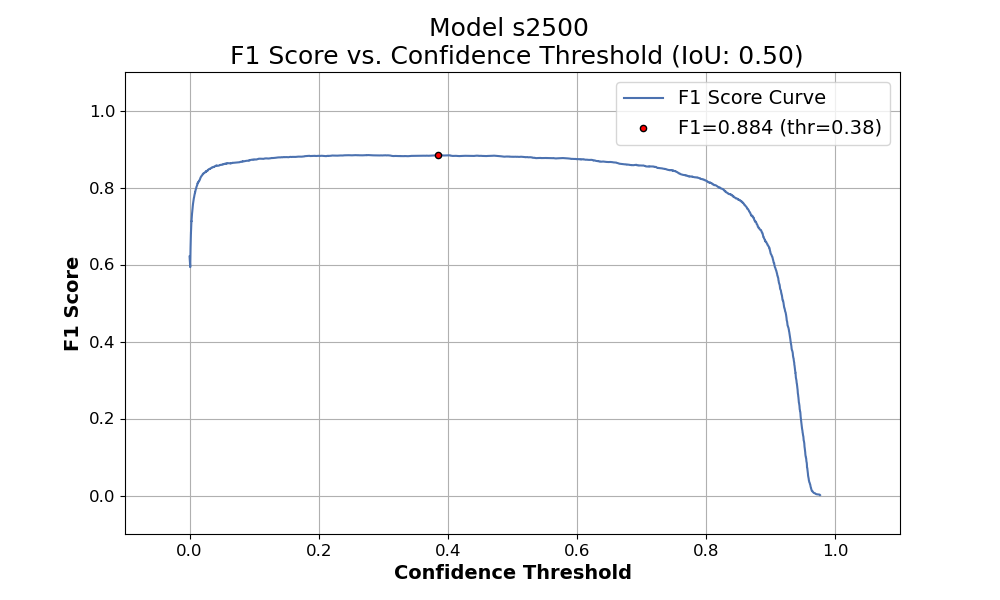
\includegraphics[width=1\textwidth]{images/results/s2500_f1_scores_0_50.png}
    \caption{F1-scores over all confidence thresholds for the s2500 model. The highest F1-score on the curve is marked with a dot.}
\label{fig:s2500_f1_scores_0_50}
\end{figure}


\begin{sidewaystable}[ht]
    \caption{Comparison between the fine-tuned YOLOv8n models and the base model. The numbers of predicted boxes, true positives (TP), false positives (FP), false negatives (FN), and derived metrics (precision, recall, and F1) are reported at each model's optimal confidence threshold. The Average Precision (AP\textsubscript{IoU:0.50}) is calculated as the area under the precision-recall curve across all confidence thresholds (0-1). All results are computed using an IoU threshold of 0.5.}
\label{tab:object_detection_metrics}
    \centering
    \Large
    \renewcommand{\arraystretch}{1.15}
    \setlength{\tabcolsep}{6pt}
\newcommand{\thdr}[1]{\shortstack[t]{\rule{0pt}{2.6ex}#1}}
\resizebox{\textheight}{!}{%
\begin{tabular}{|l|r|r|r|r|r|r|r|r|r|r|}
\hline
\thdr{Model \\ (s = synthetic, r = real)} &
\thdr{Best confidence \\ threshold} &
\thdr{Ground-truth \\ boxes} &
\thdr{Predicted \\ boxes} &
\thdr{True positives \\ (TP\textsubscript{IoU:0.50})} &
\thdr{False positives \\ (FP\textsubscript{IoU:0.50})} &
\thdr{False negatives \\ (FN\textsubscript{IoU:0.50})} &
\thdr{Precision\textsubscript{IoU:50}\\ \phantom{a}} &
\thdr{Recall\textsubscript{IoU:0.50}\\ \phantom{a}} &
\thdr{F1\textsubscript{IoU:0.50}\\ \phantom{a}} &
\thdr{AP\textsubscript{IoU:0.50}\\ \phantom{a}} \\ \hline

s500         & 0.770 & 1785 & 1747 & 1455 & 292 & 330 & 0.833 & 0.815 & 0.824 & 0.866 \\ \hline
s1000        & 0.593 & 1785 & 1748 & 1527 & 221 & 258 & 0.874 & 0.855 & 0.864 & 0.888 \\ \hline
s1500        & 0.498 & 1785 & 1789 & 1540 & 249 & 245 & 0.861 & 0.863 & 0.862 & 0.889 \\ \hline
s2000        & 0.384 & 1785 & 1702 & 1542 & 160 & 243 & 0.906 & 0.864 & 0.884 & 0.908 \\ \hline
s2500        & 0.369 & 1785 & 1654 & 1485 & 169 & 300 & 0.898 & 0.832 & 0.864 & 0.876 \\ \hline
r200         & 0.818 & 1785 & 1780 & 1384 & 396 & 401 & 0.778 & 0.775 & 0.776 & 0.828 \\ \hline
r200s500     & 0.505 & 1785 & 1531 & 1395 & 136 & 390 & 0.911 & 0.782 & 0.841 & 0.862 \\ \hline
r200s1000    & 0.398 & 1785 & 1670 & 1496 & 174 & 289 & 0.896 & 0.838 & 0.866 & 0.893 \\ \hline
r200s1500    & 0.392 & 1785 & 1622 & 1499 & 123 & 286 & 0.924 & 0.840 & 0.880 & 0.915 \\ \hline
r200s2000    & 0.441 & 1785 & 1750 & 1585 & 165 & 200 & 0.906 & 0.888 & 0.897 & 0.920 \\ \hline
r200s2500    & 0.180 & 1785 & 1771 & 1590 & 181 & 195 & 0.898 & 0.891 & 0.894 & 0.922 \\ \hline
r400         & 0.659 & 1785 & 1973 & 1520 & 453 & 265 & 0.770 & 0.852 & 0.809 & 0.854 \\ \hline
r400s500     & 0.577 & 1785 & 1604 & 1458 & 146 & 327 & 0.909 & 0.817 & 0.860 & 0.909 \\ \hline
r400s1000    & 0.609 & 1785 & 1705 & 1574 & 131 & 211 & 0.923 & 0.882 & 0.902 & 0.938 \\ \hline
r400s1500    & 0.311 & 1785 & 1738 & 1577 & 161 & 208 & 0.907 & 0.883 & 0.895 & 0.921 \\ \hline
r400s2000    & 0.228 & 1785 & 1749 & 1582 & 167 & 203 & 0.905 & 0.886 & 0.895 & 0.925 \\ \hline
r400s2500    & 0.469 & 1785 & 1721 & 1580 & 141 & 205 & 0.918 & 0.885 & 0.901 & 0.932 \\ \hline
r568         & 0.566 & 1785 & 1646 & 1540 & 106 & 245 & 0.936 & 0.863 & 0.898 & 0.923 \\ \hline
r568s500     & 0.195 & 1785 & 1746 & 1587 & 159 & 198 & 0.909 & 0.889 & 0.899 & 0.929 \\ \hline
r568s1000    & 0.350 & 1785 & 1723 & 1564 & 159 & 221 & 0.908 & 0.876 & 0.892 & 0.916 \\ \hline
r568s1500    & 0.338 & 1785 & 1694 & 1555 & 139 & 230 & 0.918 & 0.871 & 0.894 & 0.917 \\ \hline
r568s2000    & 0.218 & 1785 & 1734 & 1591 & 143 & 194 & 0.918 & 0.891 & 0.904 & 0.921 \\ \hline
r568s2500    & 0.332 & 1785 & 1714 & 1591 & 123 & 194 & 0.928 & 0.891 & 0.909 & 0.938 \\ \hline
yolov8n      & 0.161 & 1785 & 1496 & 1207 & 289 & 578 & 0.807 & 0.676 & 0.736 & 0.815 \\ \hline
\end{tabular}
}
\end{sidewaystable}

